%% LyX 2.3.6.1 created this file.  For more info, see http://www.lyx.org/.
%% Do not edit unless you really know what you are doing.
\documentclass[english,british]{article}
\usepackage[T1]{fontenc}
\usepackage[latin9]{inputenc}
\usepackage{geometry}
\geometry{verbose,tmargin=2cm,bmargin=2cm,lmargin=1cm,rmargin=1cm}
\usepackage{babel}
\usepackage{float}
\usepackage{amsmath}
\usepackage{amsthm}
\usepackage{amssymb}
\usepackage{graphicx}
\usepackage{setspace}
\doublespacing
\usepackage[unicode=true]
 {hyperref}

\makeatletter
%%%%%%%%%%%%%%%%%%%%%%%%%%%%%% User specified LaTeX commands.
\usepackage{indentfirst}
\usepackage{mathtools}

\makeatother

\begin{document}
\title{Study of liquid and nematic phases in hard spherocylinders}
\author{Leonardo H�gens and Johanna L�mker}
\maketitle
\begin{abstract}
In this project we studied a system of hard spherocylinders using
NVT and NPT Monte Carlo msimulations. We used the paper \emph{Tracing
the phase boundaries of hard spherocylinders }(Bolhuis and Frenkel,
1997) as a reference, trying to replicate some of its results. What
we found was that (...)
\end{abstract}

\section{Introduction}

The model we study in this project is the hard spherocylinders model,
and the interest in their study comes from their capability to form
all sorts of order phases, each of them mainly characterized by order/disorder
in their position and orientation, e.g. the liquid phase is the most
disordered and isotropic, while in the solid phase every spherocylinder
shares the same orientation, and they are positioned in layers orthogonal
to theirs orientation. 

The main reference we used to compare our results to was \emph{Tracing
the phase boundaries of hard spherocylinders }(Bolhuis and Frenkel,
1997) \cite{paper1}. Our first goal was to use Monte Carlo NVT simulations
to observe some of the phases of the hard spherocylinders, mainly
the liquid and nematic ones, and checking if their existence with
the used parameters makes sense according to the phase diagrams present
in \cite{paper1}. Our second goal was to use NPT Monte Carlo simulations
to build an volume-pressure state curve, as the paper has several
of them for us to compare with. During these simulations, we pay close
attention to the nematic order parameter $S$, which we'll define
later, that measures whether or not the spherocylinders have an overall
common orientation.

\section{Model}

The model we study in this project is the hard spherocylinder model,
which consists of $N$ cylinders of length $L$ that have half spheres
of diameter $D$ attached to each of its ends, whose interaction potential
is infinite if there is an overlap or touch between two of them and
vanished if there are no overlaps. The volume of a spherocylinder
is thus 
\[
v_{0}=\pi\left(\frac{LD^{2}}{4}+\frac{D^{3}}{6}\right).
\]

The particles are contained in a box of volume $V$ with periodic
boundary conditions. The convention used in \cite{paper1} and which
we'll use for the density in our project will be to use the reduced
density $\rho^{*}$, defined as 
\[
\rho^{*}=\frac{\rho}{\rho_{\text{cp}}},
\]

where $\rho_{\text{cp}}=\frac{2}{\sqrt{2}+\left(L/D\right)\sqrt{3}}$
and 
\[
\rho=\frac{Nv_{0}}{V}.
\]

To measure the orientation order/disorder of the system, we'll refer
to the nematic order parameter $S$, defined by 
\[
S=\frac{1}{N}\sum_{i=1}^{N}\left[\frac{3}{2}\cos^{2}\left(\theta_{i}\right)-\frac{1}{2}\right]
\]

where $\theta_{i}$ is the angle formed by the orientation vector
of particle $i$, $\boldsymbol{n}_{i}$, and the \emph{director} vector
$\boldsymbol{n}_{d}$, which is the normalized average of all the
orientation vectors, so:
\[
\cos\left(\theta_{i}\right)=\boldsymbol{n}_{i}\cdot\boldsymbol{n}_{d}=\boldsymbol{n}_{i}\cdot\frac{\sum_{j=1}^{N}\boldsymbol{n}_{j}}{\left|\left|\sum_{j=1}^{N}\boldsymbol{n}_{j}\right|\right|}
\]

In the case where all the particles have that same orientation, i.e.
$\boldsymbol{n}_{i}=\boldsymbol{n}\,\,\forall\,i$, we have $\cos\theta=1$,
which implies $S=1$. 

In the NPT simulations, we'll use the quantity $\beta Pv_{0}$ as
a proxy for the pressure $P$, and temperature $\beta$. 

\section{Methods}

\subsection{Minimum distance between $\left(L,D\right)$ spherocylinders}

To perform our simulations, we need to be able to check for overlapping
spherocylinders in a numeric way. To this end, we implemented the
algorithm described in \emph{A fast algorithm to evaluate the shortest
distance between rods }(Vega and Lago, 1994) \cite{paper2}. The minimum
distance this algorithm returns refers two one dimensional (thick-less)
rods, and thus two spherocylinders overlap if this distance is equal
or less than $D$.

\subsection{Visualization}

In order to observe qualitatively the phase of the system during a
simulation, we used the program \emph{Viscol}, publicly accessible
via \href{https://webspace.science.uu.nl/~herme107/viscol/}{https://webspace.science.uu.nl/~herme107/viscol/}.
In our simulation, we store each particle's position $\boldsymbol{r}_{i}$
and orientation vector $\boldsymbol{n}_{i}$, but unfortunately the
input format required by the program for it to plot the particles
is not simply the $6$ values of those two vectors. Instead, it is
required to build a rotation matrix $M$, in the picture where the
matrix acts on the frame in which the particle is fixed, and not on
the particle itself. Plugging in the identity matrix, the particle
was oriented in the $\hat{z}$ direction, which means that $M$ is
given by:
\begin{align*}
M & =R_{y}\left(-\theta\right)R_{z}\left(\phi\right)\\
 & =\left(\begin{array}{llc}
\cos\theta & 0 & -\sin\theta\\
0 & 1 & 0\\
\sin\theta & 0 & \cos\theta
\end{array}\right)\left(\begin{array}{llc}
\cos\phi & \sin\phi & 0\\
-\sin\phi & \cos\phi & 0\\
0 & 0 & 1
\end{array}\right)\\
 & =\left(\begin{array}{llc}
\cos\theta\cos\phi & \cos\theta\sin\phi & -\sin\theta\\
-\sin\phi & \cos\phi & 0\\
\sin\theta\cos\phi & \sin\theta\sin\phi & \cos\theta
\end{array}\right)
\end{align*}

where for a given orientation vector $\boldsymbol{n}$ we can determine
the elements of this matrix as follows:
\begin{align*}
\cos\theta & =\boldsymbol{n}\cdot\hat{z}\\
\sin\theta & =\sqrt{n_{x}^{2}+n_{y}^{2}}\\
\cos\phi & =\frac{n_{x}}{\sin\theta}\\
\sin\phi & =\frac{n_{y}}{\sin\theta}
\end{align*}


\subsection{NVT Monte Carlo}

To perform an NVT Monte Carlo simulation, we first pick an initial
configuration of the system, i.e. $N$ positions and orientation vectors
with no existent overlap. One initial configuration that is straightforward
to build is that of an FCC grid, for which no overlaps will exists
\emph{a priori}, and thus it is very convenient to use. In the course
of our project we did a lot of simulations, and the saved configurations
generated in NVT or NPT runs are also very convenient to use, specially
because they (the ones we studied) are mostly liquid and ranging various
densities, which if we wanted to artificially generate one liquid
configuration at a specific density it would most likely involve a
lot of inefficient trial and error. 

At each NVT MC step we pick one particle with uniform probability,
and propose to either change is position or orientation slightly,
also with uniform probability. If this displacement does not cause
the chosen particle to overlap one of its neighboring particles, we
accept it with probability of one, since the Metropolis acceptance
weight is given by
\[
\frac{\operatorname{acc}(\text{old}\rightarrow\text{new})}{\operatorname{acc}(\text{new}\rightarrow\text{old})}=\exp\left[-\beta\left(U\left(\mathbf{s}^{N};L^{\prime}\right)-U\left(\mathbf{s}^{N};L\right)+P\left(V^{\prime}-V\right)-N\beta^{-1}\ln\left(V^{\prime}/V\right)\right)\right]
\]

where in our case the hard particle interaction potential $U$ makes
this acceptance ratio always $1$ in the absence of overlaps and $0$
in their presence, and in NVT the volume $V$ is kept constant.

\subsection{NPT Monte Carlo}

An NPT MC simulation differs from an NVT one in the following manner:
at each step of the simulation, we propose to change the volume of
the box containing the particles with probability $\mathbb{\mathbb{P}}_{\text{vol}}$,
by scaling the box boundaries and positions of the particles. If a
generated uniformly random number is less than $\mathbb{\mathbb{P}}_{\text{vol}}$,
we propose that scaling, otherwise a regular NVT step will be performed.
After rejecting the proposal in the case where it has overlaps, we
accept the proposal according to the probability:
\[
\frac{\operatorname{acc}(o\rightarrow n)}{\operatorname{acc}(n\rightarrow o)}=\exp\left[-\beta P\left(V^{\prime}-V\right)+N\ln\left(V^{\prime}/V\right)\right]
\]


\section{Results and Discussions}

sdf
\begin{figure}[H]
\begin{centering}
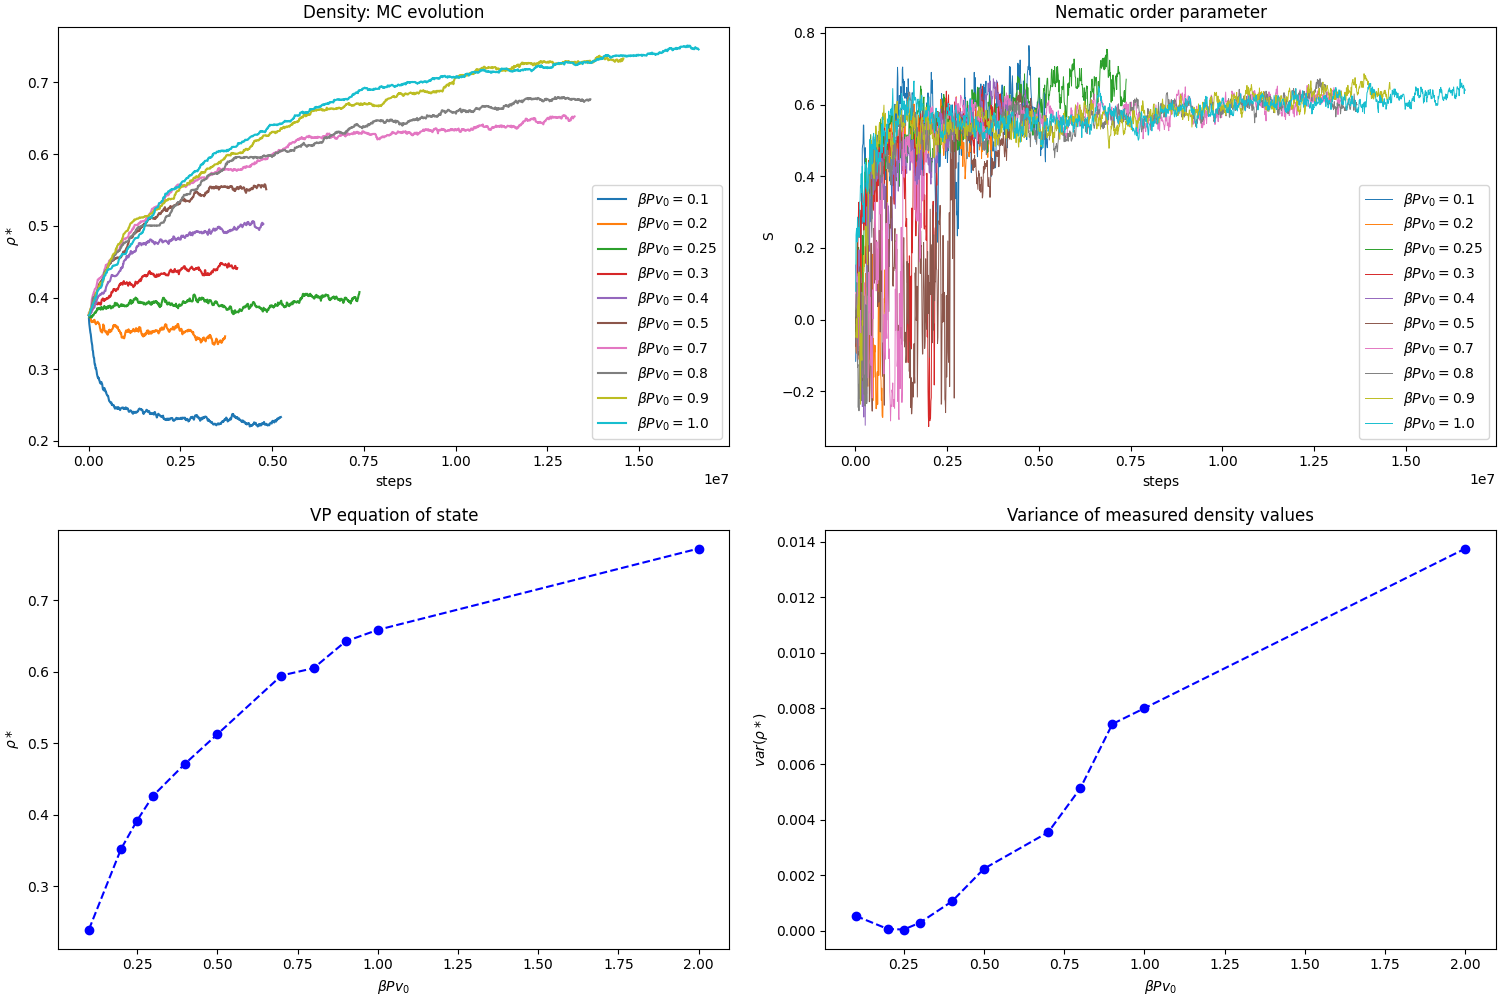
\includegraphics[width=1\textwidth]{/home/hugens/shared/uni/modsim/modsim/project/figures/NPT}
\par\end{centering}
\caption{NPT}

\end{figure}

\selectlanguage{english}%
\bibliographystyle{plain}
\nocite{*}
\bibliography{hs}
\selectlanguage{british}%

\end{document}
